\documentclass[border=10pt]{standalone}
\usepackage{tikz}
\usetikzlibrary{positioning, chains, arrows.meta, calc}
\usepackage{fontawesome}
\begin{document}
\begin{tikzpicture}[
  every node/.style = {font=\footnotesize},
  node distance     = 3em and 1em,
  every join/.style = {Latex-},
  block/.style = {draw, rounded corners, align=center,
                  minimum height=3em, minimum width=6em},
  icon/.style  = {font=\Large, minimum height=3em, inner sep=0},
  framing/.style  = {block, fill=blue!10},
  arq/.style      = {block, fill=blue!25},
  crc/.style      = {block, fill=lime!30},
  mod/.style      = {block, fill=red!15},
  preamble/.style = {block, fill=green!20},
  pulse/.style    = {block, fill=red!10},
  sdr/.style      = {block, fill=violet!15},
  decim/.style    = {block, fill=yellow!25},
  costas/.style   = {block, fill=orange!15},
  coding/.style   = {block, fill=teal!20},
  channel/.style  = {block, fill=gray!15},
  arr/.style      = {-Latex},
]
\begin{scope}[start chain=rx going right]
\node [icon,    on chain]                  {\faLaptop};
\node [arq,     on chain, join]            {ARQ};
\node [framing, on chain, join]            {Frame\\Decoder};
\node [block, fill=none, on chain, join, minimum width=8em, minimum height=5em,
       path picture={
         \fill [yellow!25]
           (path picture bounding box.south west)
           rectangle
           (path picture bounding box.center |- path picture bounding box.north);
         \fill [teal!20]
           (path picture bounding box.center |- path picture bounding box.south)
           rectangle
           (path picture bounding box.north east);
         \draw [densely dashed]
           (path picture bounding box.center |- path picture bounding box.north)
           --
           (path picture bounding box.center |- path picture bounding box.south);
       }] (rx-4) {};
\node [mod,     on chain, join]            {BPSK + 8-PSK\\Demodulator};
\node [block, fill=none, on chain, join, minimum width=8em, minimum height=5em,
       path picture={
         \fill [orange!15]
           (path picture bounding box.south west)
           rectangle
           (path picture bounding box.center |- path picture bounding box.north);
         \fill [yellow!25]
           (path picture bounding box.center |- path picture bounding box.south)
           rectangle
           (path picture bounding box.north east);
         \draw [densely dashed]
           (path picture bounding box.center |- path picture bounding box.north)
           --
           (path picture bounding box.center |- path picture bounding box.south);
       }] (rx-6) {};
\node [preamble, on chain, join]            {Frame\\Sync};
\node [pulse,   on chain, join]            {RRC \\ Matched Filter};
\node [sdr,     on chain, join]            {RX};
\end{scope}
\node [rotate=90] at ($(rx-4.west)!0.5!(rx-4.center)$) {Descrambler};
\node [rotate=90] at ($(rx-4.center)!0.5!(rx-4.east)$) {LDPC Dec.};
\node [rotate=90] at ($(rx-6.west)!0.5!(rx-6.center)$) {Costas};
\node [rotate=90] at ($(rx-6.center)!0.5!(rx-6.east)$) {NDA TED};
\node [icon,     above=of rx-1] (tx-1) {\faLaptop};
\node [arq,      above=of rx-2] (tx-2) {ARQ};
\node [framing,  above=of rx-3] (tx-3) {Frame\\Constructor};
\node [block, fill=none, anchor=center, minimum width=8em, minimum height=5em,
       path picture={
         \fill [yellow!25]
           (path picture bounding box.south west)
           rectangle
           (path picture bounding box.center |- path picture bounding box.north);
         \fill [teal!20]
           (path picture bounding box.center |- path picture bounding box.south)
           rectangle
           (path picture bounding box.north east);
         \draw [densely dashed]
           (path picture bounding box.center |- path picture bounding box.north)
           --
           (path picture bounding box.center |- path picture bounding box.south);
       }] at (tx-3 -| rx-4) (tx-4) {};
\node [rotate=90] at ($(tx-4.west)!0.5!(tx-4.center)$) {Scrambler};
\node [rotate=90] at ($(tx-4.center)!0.5!(tx-4.east)$) {LDPC Enc.};
\node [mod,      above=of rx-5] (tx-5) {BPSK + 8-PSK\\Modulator};
\node [preamble, above=of rx-7] (tx-6) {Preamble};
\node [pulse,    above=of rx-8] (tx-7) {RRC\\Pulse Shape};
\node [sdr,      above=of rx-9] (tx-8) {TX};
\foreach \src/\dst in {1/2, 2/3, 3/4, 4/5, 5/6, 6/7, 7/8}
\draw [arr] (tx-\src) -- (tx-\dst);
\node [channel, anchor=west]
      at ($(tx-8.east)!0.5!(rx-9.east) + (2em, 0)$) (chan)
      {Wireless Channel};
\draw [arr] (tx-8.east) -- (tx-8.east -| chan.north) -- (chan.north);
\draw [arr] (chan.south) -- (rx-9.east -| chan.south) -- (rx-9.east);
\end{tikzpicture}
\end{document}
